\documentclass[a4paper,landscape]{article}
\usepackage[utf8]{inputenc}
\usepackage[spanish]{babel}
\usepackage[T1]{fontenc}
\usepackage{helvet}
\renewcommand{\familydefault}{\sfdefault}
\usepackage[margin=0.85cm]{geometry}
\usepackage{graphicx}
\usepackage{fancyhdr}
\usepackage[table]{xcolor}
\setlength{\headheight}{72pt}
\usepackage{hyperref}
\usepackage{array}
\usepackage{longtable}
\usepackage{tcolorbox}
\tcbuselibrary{skins}
\graphicspath{{/mnt/DataSD/sandbox/repositorio_docente/planificaciones/core_content/4239/}}

\definecolor{linkblue}{RGB}{0,0,255}

\pagestyle{fancy}
\fancyhf{}
\fancyhead[L]{\llap{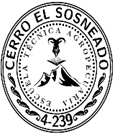
\includegraphics[height=1.5cm]{logo_esc_4239.png}}}
\fancyhead[R]{\rlap{
\includegraphics[height=1.5cm]{logo_dge_4239.png}}}
\fancyhead[C]{\begin{minipage}{12cm}\centering\fontsize{8pt}{10pt}\selectfont\bfseries\rmfamily
Escuela Nº 4-239 “Cerro el Sosneado” \\
Dirección de Educación Técnica y Trabajo \\
Paraje “El Sosneado”, San Rafael - Mendoza \\
\textcolor{linkblue}{\underline{estec4239sup@gmail.com}} \\
\fontsize{11pt}{13pt}\selectfont SUPERVISION IV – SUPERVISORA PROF. PATRICIA OROZCO
\end{minipage}}
\renewcommand{\headrulewidth}{0pt}

\begin{document}
\tcbset{colback=white, colframe=black, boxrule=0.2mm, sharp corners}


\begin{center}
\fontsize{12pt}{14pt}\selectfont\bfseries CICLO LECTIVO 2026
\end{center}

\vspace{0.5cm}
\noindent\textbf{\underline{ÁREA: TÉCNICA AGROPECUARIA}}\
\noindent\textbf{\underline{ESPACIO CURRICULAR: DIBUJO TÉCNICO}}\
\noindent\textbf{\underline{CURSO: 2do 1ra}}\
\noindent\textbf{\underline{PROFESOR/A: FERREYRA GUSTAVO DAVID}}\
\noindent PROGRAMA 2026

\vspace{0.5cm}
\begin{tabular}{|p{4cm}|p{6cm}|p{8cm}|}
\hline
\rowcolor{gray!20}\fontsize{10pt}{12pt}\selectfont\bfseries EJE TEMÁTICO & \textbf{APRENDIZAJE PRIORITARIO} & \textbf{APRENDIZAJES ESPECÍFICOS} \\ \hline
\fontsize{10pt}{12pt}\selectfont ELEMENTOS, INSTRUMENTOS Y NORMAS & Reconocer el entorno de trabajo y representar objetos aplicando normas & $\bullet$ Reconocimiento del tablero de Dibujo Técnico.\\ $\bullet$ Identificación de elementos de trazado y medición.\\ $\bullet$ Descripción del Formato de hoja.\\ $\bullet$ Aplicación de Normas I.R.A.M. generales.\\ $\bullet$ Lenguaje de comunicación técnica. \\ \hline
\fontsize{10pt}{12pt}\selectfont EJERCICIOS GEOMÉTRICOS, ESCALAS Y ACOTACIONES & Desarrollar técnicas básicas de dibujo en el plano & $\bullet$ Diagramación de formas geométricas simples.\\ $\bullet$ Interpretación y uso de escalas gráficas.\\ $\bullet$ Reconocimiento de elementos de acotación.\\ $\bullet$ Sistemas de acotación: cadena, paralelo, combinada y progresiva. \\ \hline
\fontsize{10pt}{12pt}\selectfont FORMAS DE REPRESENTACIÓN Y CROQUIZADO & Representar cuerpos 3D en el plano utilizando diversas técnicas & $\bullet$ Técnica de dibujo a mano alzada.\\ $\bullet$ Interpretación de cuerpos volumétricos.\\ $\bullet$ Técnicas de representación en el plano.\\ $\bullet$ Proyecciones de objetos reales e imaginados.\\ $\bullet$ Selección de herramientas según la situación. \\ \hline
\multicolumn{3}{|l|}{\textbf{BIBLIOGRAFÍA:}} \\ \hline
\multicolumn{3}{|l|}{$\bullet$ Normas I.R.A.M. de Dibujo Técnico.} \\ \hline
\multicolumn{3}{|l|}{$\bullet$ Manuales de Dibujo Técnico Básico.} \\ \hline
\multicolumn{3}{|l|}{$\bullet$ Guías de trabajos prácticos del espacio curricular.} \\ \hline
\end{tabular}


\end{document}